\section{Depthwise separable convolutions}

\begin{figure}[htbp]
    \centering
    \centerline{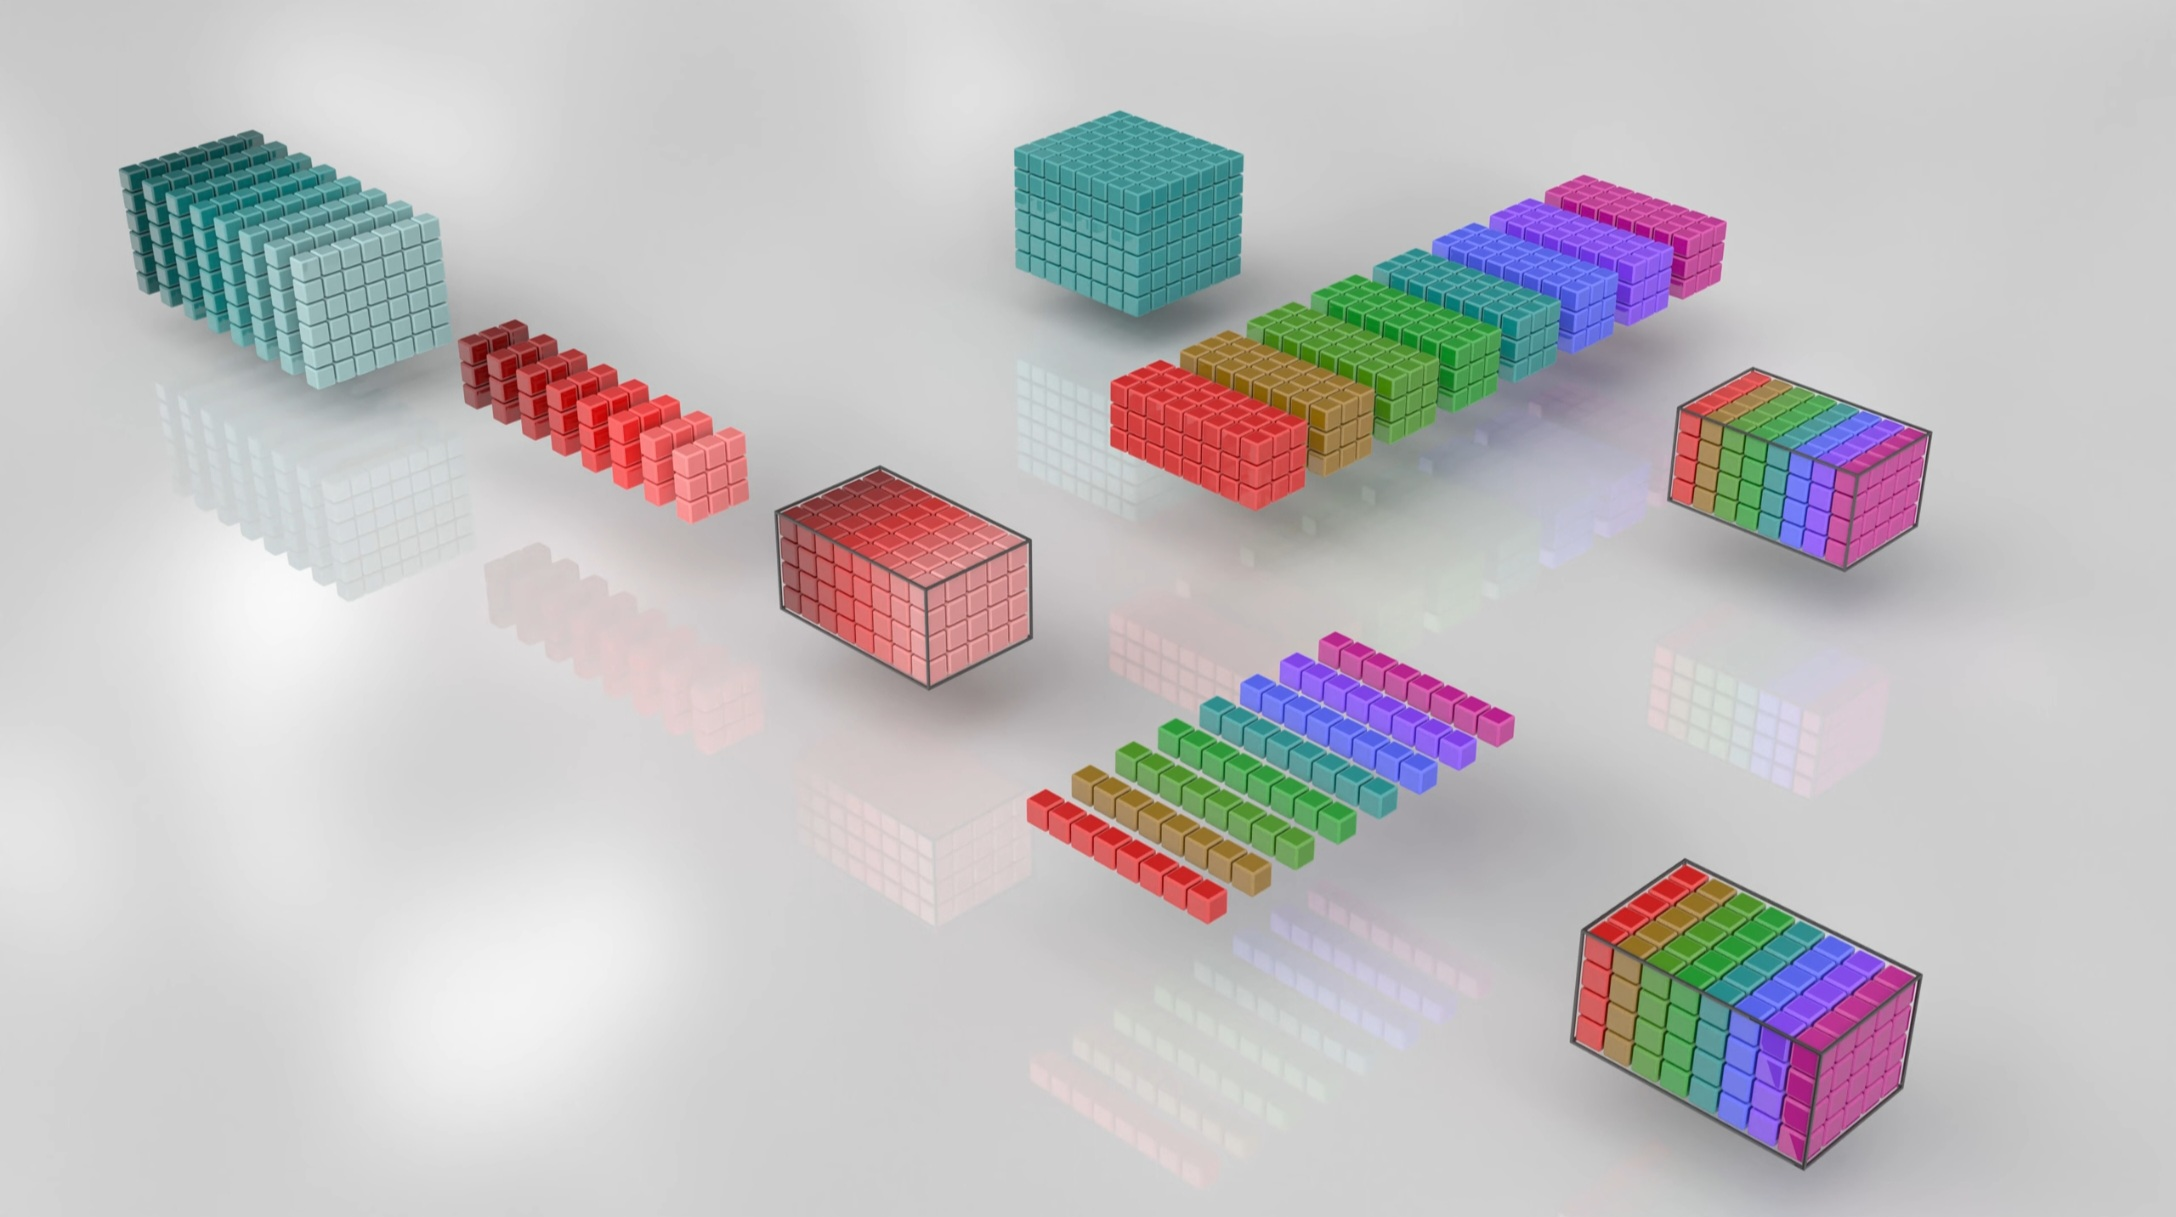
\includegraphics[width=0.8\linewidth]{images/DSC.jpg}}
    \caption{YOLO model for object detection \cite{animatedaiGroupsDepthwiseDepthwiseSeparable2023}}
    \label{fig:dsc_diagram}
\end{figure}

Figure \ref{fig:dsc_diagram} presents this comparison with depthwise separable convolutions on the left and with standard convolutional layers on the right. In a standard convolutional layer, the operation applies a 2D convolutional kernel with a size of \(K \times K\) across all input channels \(C_{in}\), resulting in a large number of parameters that need to be learned. The number of multiplications per output pixel for a standard convolution operation can be calculated as follows:
\[ Multiplications = K \times K \times C_{in} \times C_{out} \]
Depthwise separable convolutions on the other hand, splits this operation into two steps: a depthwise convolution and a pointwise convolution.

Depthwise convolution performs a spatial convolution independently on each input channel. It applies a separate filter of size \(K_d \times K_d\) that is smaller than the standard convolutional kernel to each input channel and produces an output feature map with the same number of channels as the input, which can be calculated as:
\[ Multiplications\_depthwise = K_d \times K_d \times C_{in}\]
The pointwise convolution then applies a 1x1 convolution to combine the outputs from the depthwise convolution (\(C_d\)) into the final output channels \(C_{out}\), which can be calculated as:
\[ Multiplications\_pointwise = 1 \times 1 \times C_d \times C_{out}\]
This step serves as a channel-wise linear combination and allows the network to learn complex interactions across the different channels \cite{cholletXceptionDeepLearning2017}.

Since the depthwise convolution applies a smaller number of filters to each channel independently, the number of multiplication computations required is significantly reduced as compared to a standard convolutional layer. Additionally, the pointwise convolution reduces the dimensionality of the feature maps, which further reduces the number of computations. The result, with the formula:
\[ Multiplications\_total = Multiplication\_depthwise + Multiplication\_pointwise\]
is a more computationally efficient and lightweight model that does not sacrifice too much accuracy and is better suited for deployment on devices with limited computational resources, as shown in table \ref{tab:dsccomparisons}.

\begin{table}[!htbp]
    \centering
    \caption{Model Parameter Count before and after applying depthwise separable convolutions}
    \resizebox{0.95\linewidth}{!}
    {
    \begin{tabular}{cccc}
          Model & Parameter Count & DSC Count & Reduction Percentage\\
          \hline
          baseline & 61,523,842 & 17,603,549 & 71.39\% \\
          \hline
          YOLO-BAM & 64,895,494 & 20,975,201 & 67.68\% \\
          \hline
    \end{tabular}
    }
    \label{tab:dsccomparisons}
\end{table}

However, it is important to note that depthwise separable convolutions have certain limitations or drawbacks. One such limitation is their sensitivity to input data. While these convolutions offer advantages in terms of reducing computational complexity and model size, they may struggle to capture complex spatial relationships and intricate patterns within the input data.

Due to their separable nature, depthwise separable convolutions apply separate filters to each input channel individually and then combine the results. This approach can limit the ability of the model to capture fine-grained spatial dependencies across different channels. In scenarios where the input data contains intricate spatial relationships or requires detailed feature extraction, depthwise separable convolutions may not perform as well as standard convolutions.